\documentclass[a4paper,oneside,12pt]{book}
%\documentclass[a4paper,oneside]{book}
\pagestyle{myheadings}

\setcounter{secnumdepth}{3}

%%pacote para tabela
\usepackage{booktabs}
\usepackage{graphicx}
\usepackage{adjustbox}
\usepackage[normalem]{ulem}
\useunder{\uline}{\ul}{}
\usepackage{proof,bbm}
\usepackage{stmaryrd}
\usepackage{amsmath}
\usepackage{esvect}

%%pacote de c�digos
\usepackage{listings}
\lstdefinestyle{padrao}{
	basicstyle=\ttfamily\scriptsize,
	columns=fullflexible,
	mathescape=true,
	tabsize=2, linewidth=\textwidth, 
	numbers=left,
	numberstyle=\tiny,
	stepnumber=1,
	numbersep=5pt,
	backgroundcolor=\color{gray!20},
	showspaces=false,
	showstringspaces=false,
	showtabs=false,
	frame=lines,
	tabsize=2,
	captionpos=b,
	floatplacement={tbp},
	breaklines=true,
	breakatwhitespace=false,
	escapeinside={\%*}{*)},
	numberbychapter=false
}


%%%%%%%%%%%%%%%%%%%%%%%%%%%
% Pacotes para acentua��o %
%%%%%%%%%%%%%%%%%%%%%%%%%%%

%Apenas para testar
\usepackage{cmap}
%Apenas para teste

\usepackage[brazilian]{babel}
\usepackage[utf8]{inputenc}
\usepackage[T1]{fontenc}
\usepackage{ae}
\usepackage{courier}


%%%apendice
\usepackage[titletoc]{appendix}

%%%%define uma tabela muito longa
\usepackage{longtable}

%%cor para tabela
\usepackage[table,xcdraw]{xcolor}

%%%%%%%%%%%
%\usepackage[brazilian]{babel}
\usepackage{graphicx}
\usepackage{placeins}
\usepackage{tikz}
\usepackage{amsfonts}
\usepackage{hyperref}
\usetikzlibrary{arrows,shapes,decorations,automata,backgrounds}
\usepackage{amsthm}
\usepackage{hyperref}





\usepackage{lmodern}			% Usa a fonte Latin Modern			
\usepackage[T1]{fontenc}		% Selecao de codigos de fonte.
\usepackage[utf8]{inputenc}		% Codificacao do documento (conversão automática dos acentos)
\usepackage{lastpage}			% Usado pela Ficha catalográfica
\usepackage{indentfirst}		% Indenta o primeiro parágrafo de cada seção.
\usepackage{color}		% Controle das cores
\usepackage{graphicx}			% Inclusão de gráficos
\usepackage{microtype} 			% para melhorias de justificação
\usepackage{diagbox} %tabelas com barras
% ---
		
% ---
% Pacotes adicionais, usados apenas no âmbito do Modelo Canônico do abnteX2
% ---
\usepackage{lipsum}				% para geração de dummy text
% ---

% ---
% Pacotes de citações
% ---
\usepackage[brazilian,hyperpageref]{backref}	 % Paginas com as citações na bibl
\usepackage[alf]{abntex2cite}	% Citações padrão ABNT

% --- 
% Pacotes matemáticos
% ---
\usepackage{amsthm}


% --- 
% CONFIGURAÇÕES DE PACOTES
% --- 
\newtheorem{definition}{Definição}
\newtheorem{teorema}{Teorema}
\newtheorem{corolario}{Corolário}
\graphicspath{{figuras/}}
% ---
\newtheorem{axiom}{Axioma}


\newcommand{\Mod}[1]{\ (\mathrm{mod}\ #1)}
%%%%%%%%%%%
\linespread{1.5} % espaçamento entre linhas
%%% Outros pacotes úteis - Igor - 05/11/2011
%%%%%%%%%%%%%%%%%%%%%%%%%%%%%%%%%%%%%%%%%%
%%% Insira aqui os pacotes necess�rios
%%%%%%%%%%%%%%%%%%%%%%%%%%%%%%%%%%%%%%
\usepackage{indentfirst}
\usepackage{array}

%%%%%%%%%%%%%%%%%%%%%%%%%%%%%%%%%%%%%%%%%%%%%%%%%%%%%%
%              Formata��o da P�gina                  %
%%%%%%%%%%%%%%%%%%%%%%%%%%%%%%%%%%%%%%%%%%%%%%%%%%%%%%

% horizontal
\setlength{\hoffset}{-1in}

\setlength{\oddsidemargin}{3.0cm}

\setlength{\textwidth}{160mm} % (210mm - 30mm - 20mm)

\setlength{\parindent}{1.25cm} % identa��o de cada par�grafo

% vertical
\setlength{\voffset}{-1in}
\addtolength{\voffset}{2.0cm}

\setlength{\topmargin}{0.0cm}

\setlength{\headheight}{5mm}
\setlength{\headsep}{5mm}

\setlength{\textheight}{247mm} % (297mm - 30mm - 20mm)

%\setlength{\footskip}{0mm}

%%%%%%%%%%%%%%%%%%%%%%%%%%%%%%%%%%%%%%%%%%%%%%%%%%%%%%


\begin{document}


%%%%%%%%%%%%%%%%%%%%%%%%%%%%%%%%%%%%%%%%%%%%%%%%%%%%%%
%                  Capa da Monografia                %
%%%%%%%%%%%%%%%%%%%%%%%%%%%%%%%%%%%%%%%%%%%%%%%%%%%%%%

\begin{titlepage}
  \begin{center}
    \Large{\textsc{Universidade Federal Fluminense} \\
           \textsc{Instituto de Computação} \\
           \textsc{Departamento de Ciência da Computação}
          }
    \par\vspace{3.0cm}
    \LARGE{Matheus Souza D'Andrea Alves}
%% Descomentar caso tenha outro aluno
     \par\vspace{3.0cm}
    \bigskip
    \LARGE{COLORAÇÃO DE $GRAFOS(r,l)$}
    \par\vfill
    \Large{Niterói-RJ\\2017}
  \end{center}
\end{titlepage}



%%%%%%%%%%%%%%%%%%%%%%%%%%%%%%%%%%%%%%%%%%%%%%%%%%%%%%
%                Numeracao em romano                 %
%%%%%%%%%%%%%%%%%%%%%%%%%%%%%%%%%%%%%%%%%%%%%%%%%%%%%%

\pagenumbering{roman}
\setcounter{page}{2}


%%%%%%%%%%%%%%%%%%%%%%%%%%%%%%%%%%%%%%%%%%%%%%%%%%%%%%
%                   Folha de Rosto                   %
%%%%%%%%%%%%%%%%%%%%%%%%%%%%%%%%%%%%%%%%%%%%%%%%%%%%%%


\begin{center}
Matheus Souza D'Andrea Alves


\vfill

COLORAÇÃO DE $GRAFOS(r,l)$

\vspace{3.0cm}

\begin{flushright}
\begin{minipage}{0.50\textwidth}

Trabalho submetido ao Curso de \linebreak Bacharelado em Ciência da
Computação
da Universidade Federal Fluminense como
requisito parcial para a obtenção do título de Bacharel em Ciência da
Computação.

\end{minipage}
\end{flushright}

\vspace{3.0cm}

\begin{flushleft}
Orientador: Dr. Uéverton dos Santos Souza 
\end{flushleft}

\vfill

Niterói-RJ\\2017

\end{center}

\newpage


\newpage

%%%%%%%%%%%%%%%%%%%%%%%%%%%%%%%%%%%%%%%%%%%%%%%%%%%%%%%%
%                  Dedicat�ria                                 %
%%%%%%%%%%%%%%%%%%%%%%%%%%%%%%%%%%%%%%%%%%%%%%%%%%%%%%%%

\begin{flushright}
\begin{minipage}{0.5\textwidth}

\vspace{15.0cm}
% espa�o do topo at� o in�cio da dedicat�ria



\textit{"Ignorance more frequently begets confidence than does knowledge:\\
		It is those who know little, and not those who know much,\\ who so positively assert that this or that problem\\ will never be solved by science.\\
		Charles Darwin (The Descent of Man - pg 3)}
\end{minipage}
\end{flushright}

%%%%%%%%%%%%%%%%%%%%%%%%%%%%%%%%%%%%%%%%%%%%%%%%%%%%%%%%
%                 Agradecimentos                             %
%%%%%%%%%%%%%%%%%%%%%%%%%%%%%%%%%%%%%%%%%%%%%%%%%%%%%%%%

\chapter*{Agradecimentos}

\thispagestyle{myheadings}

\noindent

[PLACE HOLDER]



%%%%%%%%%%%%%%%%%%%%%%%%%%%%%%%%%%%%%%%%%%%%%%%%%%%%
%            Resumo na l�ngua vern�cula            %
%%%%%%%%%%%%%%%%%%%%%%%%%%%%%%%%%%%%%%%%%%%%%%%%%%%%

\chapter*{Resumo}
\addcontentsline{toc}{chapter}{Resumo}

\thispagestyle{myheadings}

Um problema clássico na literatura é o problema de coloração própria de um grafo, isto é, encontrar uma q-coloração para um grafo G tal que todo vértice $v \in V(G)$ não possua nenhum vizinho da mesma cor e q seja mínimo. Esse problema é conhecido ser NP-Difícil para grafos gerais. O trabalho a seguir tem como proposta desvendar e catalogar a complexidade clássica e parametrizada de tal problema para a classe de Grafos(r,l), i.e. grafos particionáveis em r conjuntos independentes e l cliques; Identificando as características que tornam o problema difícil e a relação do problema de coloração com outros problemas, quando abordado pela perspectiva parametrizada.

\bigskip
%

\noindent Palavras-chave: \textit{Complexidade parametrizada. Grafos(r,l). Partição de grafos. Coloração de Grafos}

%%%%%%%%%%%%%%%%%%%%%%%%%%%%%%%%%%%%%%%%%%%%%%%%%%%%%%
%                      Abstract                      %
%%%%%%%%%%%%%%%%%%%%%%%%%%%%%%%%%%%%%%%%%%%%%%%%%%%%%%

\chapter*{Abstract}
\addcontentsline{toc}{chapter}{Abstract}

\thispagestyle{myheadings}
\nocite{*}

A classical problem in the literature is the problem of proper coloring a graph, i.e. to find a q-coloring for a graph G such that every vertex $ v \in V (G) $ does not have any neighbor of the same color and q is the smallest possible number, a problem known to be NP-Hard for a general graphs. The following work attempts to uncover and catalog the parametrized complexity of such problem for the class of graphs(r, l), i.e. partitionable graphs in r independent sets and l cliques; Identifying the characteristics that make the problem hard and the relation of the stated problem to other problems when approached by the parameterized perspective.

\bigskip
%

\noindent Keywords: \textit{Parametrized Complexity. Graph(r,l). Graph Partitioning. Graph Coloring. }

%%%%%%%%%%%%%%%%%%%%%%%%%%%%%%%%%%%%%%%%%%%%%%%%%%%%%%%%
%                       Sum�rio                        %
%%%%%%%%%%%%%%%%%%%%%%%%%%%%%%%%%%%%%%%%%%%%%%%%%%%%%%%%

\tableofcontents

\thispagestyle{myheadings}


%%%%%%%%%%%%%%%%%%%%%%%%%%%%%%%%%%%%%%%%%%%%%%%%%%%%%%%%
%                  Lista de Ilustra��es                %
%%%%%%%%%%%%%%%%%%%%%%%%%%%%%%%%%%%%%%%%%%%%%%%%%%%%%%%%

\listoffigures
\addcontentsline{toc}{chapter}{Lista de Figuras}

\thispagestyle{myheadings}

%%%%%%%%%%%%%%%%%%%%%%%%%%%%%%%%%%%%%%%%%%%%%%%%%%%%%%%%
%                   Lista de Tabelas                   %
%%%%%%%%%%%%%%%%%%%%%%%%%%%%%%%%%%%%%%%%%%%%%%%%%%%%%%%%

\listoftables
\addcontentsline{toc}{chapter}{Lista de Tabelas}

\thispagestyle{myheadings}


%%%%%%%%%%%%%%%%%%%%%%%%%%%%%%%%%%%%%%%%%%%%%%%%%%%%%%
%                Numeracao em arabico                %
%%%%%%%%%%%%%%%%%%%%%%%%%%%%%%%%%%%%%%%%%%%%%%%%%%%%%%

\pagebreak
\pagenumbering{arabic}

%%%%%%%%%%%%%%%%%%%%%%%%%%%%%%%%%%%%%%%%%%%%%%%%%%%%%%%%
%                       Texto                          %
%%%%%%%%%%%%%%%%%%%%%%%%%%%%%%%%%%%%%%%%%%%%%%%%%%%%%%%%




%%% Separe cada cap�tulo em um arquivo separado
%%% Os arquivos podem ter qualquer nome
\chapter{Introdução} \label{cap:introducao}
\chapter{Preparação da pesquisa}
\chapter{Análise clássica para coloração em Grafos$(r,\ell)$}
\section{Conceitos básicos}
    \subsection{Grafos$(r,\ell)$}
     \begin{definition}
         Um Grafo dito Grafo$(r,\ell)$ ou abreviadamente $G(r,\ell)$ é qualquer grafo pertencente á classe dos grafos que podem ser particionados em r conjuntos independentes e l cliques.
     \end{definition}
    \subsection{Coloração mínima de Grafos}
     \begin{definition}
         Entrada: um Grafo $G$ e um inteiro $k$\\
  Questão: Cada vértice pertencente à $G$ pode ser colorido com uma entre $k$ cores
  de tal forma que dado quaisquer dois vértices adjacentes eles tenham cores distintas e $k$ seja o mínimo de cores possível?
     \end{definition}

\section{Exploração do problema de coloração mínima em Grafos$(r,\ell)$}
    O problema de coloração aplicado a Grafos$(r,\ell)$ é de fácil solução para algumas especificações,
por exemplo um Grafo vazio, que é um Grafo(0,0) pode ser colorido com 0 cores, um Grafo disperso i.e um Grafo(1,0) é colorível com apenas uma cor, já que não existem arestas nesse grafo.

Já um Grafo completo, ou seja um Grafo(0,1), é colorível com K cores onde K é a quantidade de vértices nesse grafo completo, em um Grafo split que é um Grafo(1,1) essa regra se repete, já que cada vértice do conjunto independete pode ser colorível com alguma cor já presente na clique.

E por fim, Grafos bipartidos são coloridos com 2 cores uma cor para cada conjunto independente.

Sabemos então que coloração é de solução polinomial para grafos completos, dispersos, split e para grafos bipartidos. Assim, temos como ponto de partida para a exploração futura da complexidade de Grafos de cardinalidade superiores a seguinte tabela.

%primeira tabela de dicotomia
\begin{table}[htb!]
  \center
  \begin{tabular}{l|*{7}c}
    \toprule
    \backslashbox{$r$}{$l$} & 0 & 1 & 2 & 3 & 4 & \ldots & n\\
    \midrule
    0 & \textit{P} & \textit{P} & ? & ? & ? & \ldots & ?\\
    1 & \textit{P} & \textit{P} & ? & ? & ? & \ldots & ?\\
    2 & \textit{P} & ? & ? & ? & ? & \ldots & ?\\
    3 & ? & ? & ? & ? & ? & \ldots & ?\\
    4 & ? & ? & ? & ? & ? & \ldots & ?\\
    $\vdots$ & $\vdots$ & $\vdots$ & $\vdots$ & $\vdots$ & $\vdots$ & $\ddots$ & ?\\
    n & ? & ? & ? & ? & ? & \ldots & ?\\
    \bottomrule
  \end{tabular}%
  \caption{1ª Dicotomia parcial do problema de coloração em Grafos$(r,\ell)$}
  \label{tab:tabela_part1dictrl}%
\end{table}%


Portanto agora nos é interessante abordar a complexidade para as classes na fronteira do que já conheçemos
%Teorema que coloração em (3,0) e (0,2) são polinomiais e (4,0) é NPc 
\begin{itemize}
  \item Grafo(0,2):
     \begin{teorema}
        Coloração de Grafo(0,2) é Polinomial.
     \end{teorema}
     \begin{proof}
      Um Grafo(0,2) é um grafo separável em 2 cliques, e que todo vértice faz parte de alguma das cliques, logo conhecer a clique máxima é simples e tendo a clique máxima sabemos que o numero mínimo de cores que pode ser usado para colorir o grafo é a cardinalidade da clique máxima.
     \end{proof}
  \item Grafo(3,0):
     \begin{teorema}
        Coloração de Grafo(3,0) é Polinomial.
     \end{teorema}
     \begin{proof}
      Tendo um Grafo G da classe (3,0) como entrada para o problema de coloração sabemos então que o grafo pode ser colorido com 3 cores, resta saber se 3 é o o número mínimo de cores que pode ser usado, portanto devemos verificar se G é bipartido (colorível com duas cores) ou um grafo sem arestas (colorível com uma cor), como ambas verificações são polinomiais podemos afirmar que coloração de Grafo(3,0) é resolvível de forma polinomial.
     \end{proof}
  \item Grafo(4,0):
      \begin{teorema}
        Coloração de Grafo(4,0) é NP-Completo.
      \end{teorema}
      \begin{proof}
        Sabemos que todo grafo planar é 4-colorível, e que alguns Grafos(4,0) são planares, portanto sabemos que para qualquer Grafo G $\in$ subconjunto de planares de Grafos(4,0), sua quantidade máxima de cores é 4, nos resta saber se 4 também é sua quantidade mínima, porém 3-coloração de planar é NP-Completo logo descobrir a coloração mínima de G é NP-Completo e consequentemente coloração de Grafos(4,0) é NP-Completo
      \end{proof}
\end{itemize}

É importante notar aqui que, todo $Grafo(r,\ell)$ é simultaneamente um $Grafo(r,\ell+1)$ já que podemos formar uma nova clique trivial utilizando qualquer vértice, e um $Grafo(r+1,\ell)$ já que podemos formar um novo conjunto independente trivial a partir de qualquer vértice, portanto se o problema de coloração é NP-Completo para um $Grafo(r,\ell)$ então ele é NP-Completo para qualquer $Grafo(r+1,\ell)$ ou $Grafo(r,\ell+1)$ .

Esses resultados nos levam à preencher a dicotomia da seguinte forma
%Segunda tabela de dicotomia
\begin{table}[htb!]
  \center
  \begin{tabular}{l|*{7}c}
    \toprule
    \backslashbox{$r$}{$l$} & 0 & 1 & 2 & 3 & 4 & \ldots & n\\
    \midrule
    0 & \textit{P} & \textit{P} & \textit{P} & ? & ? & \ldots & ?\\
    1 & \textit{P} & \textit{P} & ? & ? & ? & \ldots & ?\\
    2 & \textit{P} & ? & ? & ? & ? & \ldots & ?\\
    3 & \textit{P} & ? & ? & ? & ? & \ldots & ?\\
    4 & \textit{NPc} & \textit{NPc} & \textit{NPc} & \textit{NPc} & \textit{NPc} & \ldots & \textit{NPc}\\
    $\vdots$ & $\vdots$ & $\vdots$ & $\vdots$ & $\vdots$ & $\vdots$ & $\ddots$ & \textit{NPc}\\
    n & \textit{NPc} & \textit{NPc} & \textit{NPc} & \textit{NPc} & \textit{NPc} & \ldots & \textit{NPc}\\
    \bottomrule
  \end{tabular}%
  \caption{2ª Dicotomia parcial do problema de coloração em Grafos$(r,\ell)$}
  \label{tab:tabela_part2dictrl}%
\end{table}%

Ainda nos falta mostrar a complexidade para alguns casos de fronteira, que necessitam de uma demonstração mais complexa.
%Demonstrar lista-coloração(r,l)Npc -> coloração(r,l+1)Npc e seus colorários (1,2) & (2,1)

Iremos demonstrar abaixo a complexidade para tais casos utilizando o seguinte teorema. 
    \begin{teorema}
      Coloração de Grafos$(1,2)$ é NP-Completo
    \end{teorema}
    \begin{proof}
      A prova do teorema baseia-se em mostrar que uma solução de lista coloração para grafos$(r,\ell)$ implica em uma solução para o problema de coloração de um Grafo$(r,\ell+1)$ $H_G$, portanto para provarmos é preciso mostrar que
      \begin{itemize}
        \item Se um grafo G$(r,\ell)$ possui uma lista coloração própria então $H_G$ é k-colorível para k=nº de cores nas listas (1)
        \item Se $H_G$ é k-colorível então G possui uma lista coloração própria (2)
      \end{itemize}
      (1):\newline
      
      Usaremos a seguinte construção:\newline
      Considere G um grafo$(r,\ell)$ e que para cada vértice $v \in V(G)$ exista uma lista de cores $S_v$ referente a esse vértice, cada lista contém pelo menos uma cor do conjunto $C = \{c_1,c_2,c_3,...,c_k \}$, sendo G uma instância sim para o problema de lista coloração, criemos uma clique K onde cada vértice $k \in V(K)$ representa uma cor presente em $C$. Seja $H_G = G \cup K$ para todo vértice $v \in G$ e todo vértice $u_i \in K$ adicione uma aresta $(u_i,v)$ à $H_G$ se e somente se v não possui a cor $c_i$ em sua lista coloração em G
      
      Podemos então generalizar da seguinte forma, dado um grafo$(r,\ell)$ $G$ onde cada vértice de $G$ possui uma lista de possíveis cores então o grafo $H_G$ obtido pela construção anterior possui uma k-coloração.
      
      Note que a clique K possui exatamente k vértices, consequentemente para colorirmos K precisaremos de k cores, sem perda de generalidade assumimos que $u_1$ será colorido com $c_1$, $u_2$ com $c_2$ e assim por diante.
      
      Por construção uma aresta de $u_i$ só existe para $v_a$ em $H_G$ se e somente se, $v_a$ não possui $c_i$ em sua lista de cores, portanto a coloração atribuída à K não conflita com a com a lista coloração de G, e portanto para todo vértice perntecente a G podemos lhe atribuir a mesma cor que lhe foi atribuída no problema de lista coloração, obtendo uma coloração própria mínima para $H_G$
      
      (2):\newline
      Suponha que o grafo $H_G$ possua uma K-coloração própria, onde k é o número de cores nas listas de G
      
      Seja K a maior clique presente em $H_G$, por construção $H_G$ é colorível com k cores onde k é a cardinalidade de K, observe que a remoção de K não afeta a coloração de $H_G - K$
      
      Como $H_G$ é k-colorível e a clique K possui k vértices todas as cores de tal k-coloração estão presentes em K. Sem perda de generalidade podemos assumir que as cores $c_1,c_2,...,c_k$ estão atribuídas aos vértices $u_1,u_2,...,u_k$ pertencentes à K
      
      Por construção de $H_G$ todo par $(v,u_i)$ onde $v \in H_G - K$ e $u_i \in K$ é não adjacente se e somente se o vértice $v$ não possui $c_i$ em sua lista coloração no grafo $G$
      
      Logo a k-coloração atribuídas aos vértices em $H_G - K$ formam uma coloração para G onde todo vértice em $V(G)$ possui uma cor de sua lista. Portanto G é uma instância sim de lista coloração
    \end{proof}
    \begin{corolario}
     Se lista coloração é NP-Completo para Grafos split então coloração é NP-Completo para Grafos$(1,2)$.
     \begin{proof}
     A NP-Completude de lista coloração em grafos split é demonstrado por Jensen et al.\cite{jansen1997}
     \end{proof}
    \end{corolario}
    \begin{corolario}
    Se Lista coloração é NP-Completo em Grafos(2,0) então Coloração é NP-Completo em Grafos$(2,1)$.
    \begin{proof}
    A NP-Completude de lista coloração em grafos bipartido é demonstrado por Fellows et al. em "List Coloring and Precoloring Extension are W[1]-hard parameterized by treewidth"
    \end{proof}
    \end{corolario}    
    \begin{corolario}
    Se lista coloração é NP-Completo para Grafos(0,2) então Coloração é NP-Completo em Grafos(0,3).
    \begin{proof}
    Para essa demonstração nos basearemos em um resultado obtido por Jensen em "Complexity results for the optimum cost chromatic partition problem". a demonstração se baseia em realizar uma redução do problema 3-SAT restrito para lista coloração de co-bipartido i.e. Grafo(0,2).
    Suponha o problema 3-SAT com as seguintes restrições:
    \begin{itemize}
      \item cada cláusula $c_i$ contém dois ou três literais.
      \item cada literal ou sua negação aparece no máximo em 3 cláusulas
    \end{itemize}
    Construiremos agora uma instância de lista coloração da seguinte forma:\newline
    Para cada varíavel $j$ crie seis vértices:
    $a_j^{(1)}$, $a_j^{(2)}$, $a_j^{(3)}$;
    $b_j^{(1)}$, $b_j^{(2)}$, $3_j^{(3)}$. Atribuindo a cada uma lista de cores da seguinte forma:\newline
    $a_j^{(k)}$ <= \{$x_j^{(k)}$, $\overline{x_j}^{(k)}$ \}; $b_j^{(k)}$ <= \{$\overline{x_j}^{(k)}$,$x_j^{((k \Mod{3}) + 1 )}$ \}\newline
    Definimos como A o conjunto de todos os $a_j^{(k)}$ e B o conjunto de todos os $b_j^{(k)}$ e construímos uma clique com os vértices de A e B. Observe que só existem duas maneiras de se colorir este grafo:
    \begin{itemize}
      \item (1)  $f(a_j^{(k)}) = x_j^{(k)} => b_j^{(k)} = \overline{x_j}^{(k)}$
      \item (2)  $f(a_j^{(k)}) = \overline{x_j}^{(k)} => b_j^{(k)} = x_j^{((k \Mod{3}) + 1 )}$
    \end{itemize}
    Agora, para cada cláusula definimos um vértice $c_i$ e sua lista de cores da seguinte forma: para cada literal $j$ ou sua negação $\overline{j}$ presente na cláusula adicionamos à lista de $c_i$ o $x_j^{(k)}$ onde k é o indice de ocorrência do literal ou de sua negação.
    
    Por exemplo, suponha o seguinte 3-SAT:
    
    $(p \lor q \lor r) \land (\neg{p} \lor q \lor r) \land (\neg{p} \lor \neg{r} \lor s)$
    
    suas cláusulas seriam traduzidas para
    \begin{itemize}
      \item $c_1$ com lista: \{$p^1$, $q^1$, $r^1$ \}
      \item $c_2$ com lista: \{$\overline{p}^2$, $q^2$, $r^2$ \}
      \item $c_3$ com lista: \{$\overline{p}^3$, $\overline{r}^3$, $s^1$ \}
    \end{itemize}
    Seja C o conjunto contendo todos os $c_i$ criamos uma clique com $C \cup A$.
    Nosso grafo tem portanto a seguinte configuração(considere $x'$ como $\overline{x}$):
    \begin{figure}[!ht]
        \centering
        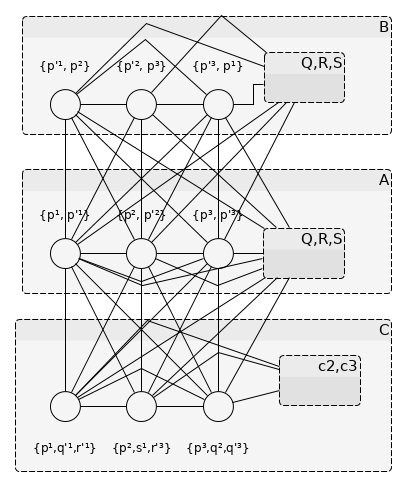
\includegraphics[width=0.6\textwidth]{3-SAT.png}
        \caption{Grafo G: Transformaçao de 3-SAT em co-bipartido }
      \end{figure}
      
      Suponha a cláusula p, se p é falso então $a_p^{(1)},a_p^{(2)},a_p^{(3)}$ será colorido com $p^1,p^2,p^3$ respectivamente
      
    Dessa forma mostramos que o o grafo construído só tem solução para lista coloração se existe pelo menos um literal verdadeiro em todas as cláusulas
    \end{proof}
    \end{corolario}
    
Portanto podemos agora completar nossa tabela com:

\begin{table}[htb!]
  \center
  \begin{tabular}{l|*{7}c}
    \toprule
    \backslashbox{$r$}{$l$} & 0 & 1 & 2 & 3 & 4 & \ldots & n\\
    \midrule
    0 & \textit{P} & \textit{P} & \textit{P} & \textit{NPc} & \textit{NPc} & \ldots & \textit{NPc}\\
    1 & \textit{P} & \textit{P} & \textit{NPc} & \textit{NPc} & \textit{NPc} & \ldots & \textit{NPc}\\
    2 & \textit{P} & \textit{NPc} & \textit{NPc} & \textit{NPc} & \textit{NPc} & \ldots & \textit{NPc}\\
    3 & \textit{P} & \textit{NPc} & \textit{NPc} & \textit{NPc} & \textit{NPc} & \ldots & \textit{NPc}\\
    4 & \textit{NPc} & \textit{NPc} & \textit{NPc} & \textit{NPc} & \textit{NPc} & \ldots & \textit{NPc}\\
    $\vdots$ & $\vdots$ & $\vdots$ & $\vdots$ & $\vdots$ & $\vdots$ & $\ddots$ & \textit{NPc}\\
    n & \textit{NPc} & \textit{NPc} & \textit{NPc} & \textit{NPc} & \textit{NPc} & \ldots & \textit{NPc}\\
    \bottomrule
  \end{tabular}%
  \caption{Dicotomia do problema de coloração em Grafos$(r,\ell)$}
  \label{tab:tabela_dictrl}%
\end{table}%

\chapter{Análise parametrizada para coloração em Grafos(2,1)}
Tendo mostrado a complexidade clássica nos é interessante agora que elucidemos quais caractéristicas dos grafos(r,l) se mostram propícias a abordagem parametrizada, a cardinalidade de suas partições se mostrou uma interesante característica.
Decidimos abordar a classe (2,1), já que a mesma é a classe onde o problema é NP-Completo com o menor número de partições.

Um Grafo(2,1) é um grafo particionado em 2 conjuntos independentes e 1 clique, portanto ele nos entrega 3 naturais candidatos a parametrização, o tamanho da clique $l$, o tamanho do menor conjunto independente $r_1$ e o tamanho do maior conjunto independente $r_2$.

\section{Parametrização pelo tamanho do menor conjunto independente}
Em \ref{Fellows07} Fellows (et. al) mostrou que o problema de lista coloração é $W[1]-difícil$ parametrizado pela treewidth através da transformação do problema da clique multicolorida parametrizada pelo tamanho da clique para tal, nos aproveitaremos dessa transformação para mostrar que:
\begin{teorema}
O problema de coloração em Grafos(2,1) é $W[1]-difícil$ quando parametrizado pelo tamanho do menor conjunto independente.
\end{teorema}
\begin{proof}
Observe a seguinte transformação.

O problema da clique multicolorida pode ser definido como: Dado um Grafo $G$ detentor de uma $k-coloração$ própria, existe uma clique de tamanho $k$ abrangendo todas as cores? Esse problema é conhecidamente $W[1]-difícil$.

Portanto suponha tal $G$ proposto, temos como intenção montar um problema de lista coloração em um grafo $G'$ a partir dele, para tanto seguimos os seguintes passos:
\begin{itemize}
  \item Para cada cor $i$ presente em $G$ cria-se em $G'$ um vértice $v_i$ (os chamaremos de vértices-cor).
  \item Para cada vértice $u$ em $G$ colorido com a cor $i$, adicionamos à lista do vértice-cor $v_i$ em $G'$ uma cor $c_u$ relacionada a esse vértice (as chamaremos de cores-vértice).
  \item Para cada aresta $e(x,y) \notin E(G)$ onde $x,y \in V(G)$ cria-se em $G'$ um vértice $z_e$ adjacente ao vértice-cor $v_i$ onde $i$ representa as cores de $x$ e $y$, a lista coloração de $z_e$ será formada por $c_x$ e $c_y$.
\end{itemize}
É notável que a treewidth de $G'$ é dada por $k$, já que a remoção dos vértices-cor leva a um grafo sem arestas. Assim sendo se $G$ possui uma clique multicolorida podemos facilmente colorir $G'$ da seguinte forma:

Ao vértice-cor $v_i$ atribua a cor-vértice $c_u$ onde $u$ é o vértice colorido com a cor $i$ em $G$. Dessa forma todos os vértices $z_e$ possuem ainda uma cor disponível para sua coloração já que ele representa uma não-aresta em $G$. 

Para a volta observe que uma lista coloração válida em $G'$ implica em uma clique multicolorida em $G$, isso se dá pois dois vértices $x,y$ coloridos com cores diferentes em $G$ não aparecem em uma lista de algum $z_e$ em $G'$ se e somente se existe uma aresta $e(x,y) \in E(G)$, portanto as cores-vértices escolhidas para os vértices $v_i$ são uma respectivamente uma clique formadas por tais $i$ em $G$. Mostramos assim que lista coloração parametrizada por treewidth é $W[1]-difícil$.

Sabemos que coloração em Grafos(2,1) é equivalente a lista coloração em um grafo bipartido, portanto nossa tentativa de parametrizar a coloração de (2,1) pelo tamanho do menor conjunto independente é equivalente a parametrizar lista-coloração em bipartidos pelo tamanho do menor conjunto independente, é de pouca dificuldade ver que a treewidth de um grafo bipartido existe em função do menor independente, mostrando assim que coloração em Grafos(2,1) parametrizada pelo tamanho do menor conjunto independente é $W[1]-difícil$. 

\end{proof}

\section{Parametrização pelo tamanho da clique}
Para a demonstração da complexidade parametrizada utilizando $k=\#l$ nos voltamos novamente para transformação da clique em um Grafo(2,1) em listas coloração do restante bipartido, dessa forma nosso problema parametrizado original se torna um novo problema, lista coloração de bipartido parametrizado pelo tamanho da paleta de cores. 

Mostraremos no entanto que essa parametrização não é proveitosa já que o problema se mostra equivalente à PreColoring Extension com limite de cores, mostrado ser NP-Completo para grafos bipartidos mesmo quando sua paleta é de tamanho 3\cite{Kratochvil94}.

\begin{teorema}
Lista coloração em bipartidos com listas de tamanho 1 é NP-Completo
\end{teorema}
\begin{proof}
Suponha uma instância $P$ do problema PreColoring Extension e $G$ seu grafo de entrada, sabemos que $G$ possui uma paleta $C$ de cores de tamanho definido, e que existem $v \in V(G)$ que já estão coloridos com uma cor $c \in C$, podemos ver tal configuração como um grafo $G'$ onde os vértices $v$ possuem listas contendo apenas $c$, e os demais vértices possuem listas de tamanho $\#C$ contendo todas as cores, nos levando a um problema de lista coloração $Q$ que tem como entrada $G'$.

Uma coloração possível para $P$ implica em uma coloração possível para $Q$, já que nos basta atribuir aos vértices em $G'$ as mesmas cores atribuídas em $G$. Da mesma forma uma lista coloração possível em $Q$ implica em uma coloração possível em $P$.
\begin{proof}


Apesar do tamanho da paleta não ter se mostrado uma escolha adequada, ele levanta novos parametros que são interessantes para o problema de lista coloração em bipartidos, observe pois que, sabemos que Precoloring extension é polinomial se todas as listas tem tamanho 1 ou 2 \cite{HUJTER93}, e NP-Completo se todas tem listas e tamanho 1 e 3 \cite{Kratochvil94}, isso levanta duas formas de se abordar o problema, o que acontece quando o número de vértices com listas de tamanho 1 e 2 varia, e o que acontece quando o número de vertices com listas de tamanho 3 varia.

Mostraremos nas próximas seções como se dão tais comportamentos e como eles se relacionam a coloração de Grafos(r,l)
\section{O problema de lista coloração em bipartidos com paleta de tamanho 3 parametrizado pela quantidade de vértices com listas de tamanho 1 ou 2}
Subdiviremos essa seção abordando os casos em que existem apenas listas de tamanho 1, e onde existem listas de tamanho 2.
\subsection{Apenas listas de tamanho 1}
 <Não lembro como,> sabemos que precisamos de 6 vértices de tamaho 1 para que o problema se 
\section{O problema de lista coloração em bipartidos com paleta de tamanho 3 parametrizado pela quantidade de vértices com listas de tamanho 3}
Mostraremos que o problema é FPT utilizando o seguinte algoritmo de árvore de profundidade limitada.

\chapter{Análise parametrizada de problemas relacionados a coloração}
\chapter{Resultados}
\chapter{Conclusão}
%%%%%%%%%%%%%%%%%%%%%%%%%%%%%%%%%%%%%%%%%%%%%%%%%%%%%%%%%%%%%%%%%%%
%                  Referencias Bibliograficas                   %  
%%%%%%%%%%%%%%%%%%%%%%%%%%%%%%%%%%%%%%%%%%%%%%%%%%%%%%%%%%%%%%%%%%%
\cleardoublepage
\addcontentsline{toc}{chapter}{Referências Bibliográficas}

%\appendix
%\include{apendice1}
%\apendice
%\cleardoublepage
%\addcontentsline{toc}{chapter}{Ap\^endices}
%\begin{appendices}
%\chapter{Teste}
%\end{appendices}
\bibliographystyle{IEEEtran}
\bibliography{references}%{} % arquivos fonte com a bibliografia
\end{document}
